% Compilar com: latexmk -lualatex I1-covariance__sector.tex
% Tabelas e números em tab/ são gerados por ../../info_covariance_assumed_tex.py a partir do manifesto de
% info_covariance_assumed.py. Não editar números à mão: regenerar (DESIGN_SYSTEM 2.08).
\documentclass[11pt,a4paper]{article}
\usepackage[margin=2cm]{geometry}
\usepackage{fontspec}
\usepackage{unicode-math}
\setmainfont{Latin Modern Roman}
\setmathfont{Latin Modern Math}
\usepackage[brazil]{babel}
\usepackage{booktabs,tabularx,array,graphicx,float,longtable}
\usepackage{enumitem}
\usepackage{xurl}
\usepackage[colorlinks=true,linkcolor=blue!50!black,urlcolor=blue!50!black,citecolor=blue!50!black]{hyperref}
\usepackage{xcolor}
\setlength{\parindent}{0pt}
\setlength{\parskip}{0.5em}
\newcolumntype{Y}{>{\raggedright\arraybackslash}X}
\newcommand{\arq}[1]{\texttt{\nolinkurl{#1}}}
\newcommand{\caixa}[2]{\par\noindent\colorbox{#1}{\parbox{\dimexpr\linewidth-2\fboxsep}{#2}}\par}
% generated by info_covariance_assumed_tex.py from I1-covariance__sector__cs-rbf.json; do not edit
\newcommand{\valNbins}{917}
\newcommand{\valNobs}{40}
\newcommand{\valNau}{791}
\newcommand{\valNda}{126}
\newcommand{\valCsAuMean}{0{,}052}
\newcommand{\valCsAuHalf}{5{,}2}
\newcommand{\valCsAuZero}{94{,}8}
\newcommand{\valCsAuRank}{38}
\newcommand{\valCsAuEig}{6{,}8}
\newcommand{\valCsDaMean}{0{,}143}
\newcommand{\valCsDaHalf}{14{,}3}
\newcommand{\valCsDaZero}{85{,}7}
\newcommand{\valCsDaRank}{10}
\newcommand{\valCsDaEig}{20{,}6}
\newcommand{\valRho}{1}
\newcommand{\valSigCs}{a77902df73a5}
\newcommand{\valStepsCs}{200 $\times$ 50\,000}
\newcommand{\valDiffCs}{0 (idênticas)}
\newcommand{\valRbfAuMean}{0{,}008}
\newcommand{\valRbfAuHalf}{0{,}8}
\newcommand{\valRbfAuZero}{96{,}1}
\newcommand{\valRbfAuRank}{559}
\newcommand{\valRbfAuEig}{1{,}1}
\newcommand{\valRbfDaMean}{0{,}061}
\newcommand{\valRbfDaHalf}{6{,}9}
\newcommand{\valRbfDaZero}{85{,}7}
\newcommand{\valRbfDaRank}{82}
\newcommand{\valRbfDaEig}{8{,}2}
\newcommand{\valLpt}{0{,}5}
\newcommand{\valLeta}{1}
\newcommand{\valLcent}{10}
\newcommand{\valSigRbf}{a873ae558cc9}
\newcommand{\valStepsRbf}{200 $\times$ 50\,000}
\newcommand{\valDiffRbf}{0 (idênticas)}
\newcommand{\valNsectors}{48}
\newcommand{\valNsplit}{8}

\makeatletter\newcommand{\tabin}[1]{\@@input #1 }\makeatother  % primitive \input: works inside tables

\title{Covariância experimental suposta: CS sector e RBF sector\\
\large regra, parâmetros e matriz resultante}
\date{25 de novembro de 2026}
\author{Proposta 2 --- \texttt{2-Second\_sensitivity\_test\_sector} \quad (I1-covariance, tag \texttt{sector})}

\begin{document}
\maketitle
\vspace{-1.5em}

\caixa{blue!6}{\textbf{Resumo.} Na proposta 2, a correlação das incertezas experimentais é \emph{suposta} só dentro de
\textbf{setores}: um setor é o sistema, mais a chave exata do observável, mais uma região de rapidez configurada. Os
\valNobs{} observáveis (\valNbins{} bins) formam \valNsectors{} setores. Bins de setores diferentes não têm correlação.
\textbf{CS sector:} $\rho=\valRho$ entre todos os bins do mesmo setor. A matriz tem posto \valCsAuRank{} (Au-Au) e
\valCsDaRank{} (d-Au), um modo por setor.
\textbf{RBF sector:} dentro do setor, $R_{ij}=\exp[-((x_i-x_j)/L)^2]$ na coordenada diferencial do observável, com
$L_{p_T}=\valLpt$\,GeV/$c$, $L_\eta=\valLeta$ e $L_{\rm cent}=\valLcent$ p.p.
Correlação média fora da diagonal: CS $\valCsAuMean$ e RBF $\valRbfAuMean$ (Au-Au); $\valCsAuZero\%$ e $\valRbfAuZero\%$ dos
pares têm $R=0$. A diagonal é a da baseline. Da matriz em diante, o procedimento é o mesmo de todas as propostas.}

\section{Objetivo}
A verossimilhança da calibração (Mankolli \emph{et al.}, PRC 114, 014905) é
$-2\ln L=(y-\mu(\theta))^{\!\top}(\Sigma_{\rm exp}+\Sigma_{\rm emu})^{-1}(y-\mu(\theta))$. Na baseline,
$\Sigma_{\rm exp}={\rm diag}(\sigma_i^2)$. Este documento registra \textbf{a regra que gera a parte fora da diagonal} em
cada modelo da proposta 2, com todos os parâmetros, e mostra a matriz resultante em números.

\section{Dados: os observáveis da calibração}
A matriz cobre os \valNobs{} observáveis da calibração do 3dglauber, na ordem da verossimilhança
(\arq{mcmc/02_08_sector_input_correlations/bin_index.csv}). As incertezas estão no espaço da verossimilhança:
\begin{equation}
\sigma_i=\sqrt{\ln\!\big(1+(\sigma^{\rm exp}_i/y_i)^2\big)}\ \ (dN/d\eta),\qquad \sigma_i=\sigma^{\rm exp}_i\ \ (\text{demais}).
\end{equation}
Os valores bin a bin estão no Apêndice~\ref{ap:sigma}. Para todo modelo, $\Sigma_{ij}=\sigma_i\sigma_j R_{ij}$ com
$R_{ii}=1$: \textbf{só a correlação $R$ muda}.

\section{Método}
\subsection{Setores}
O setor de um bin é \emph{(sistema, chave exata do observável, rótulo da região de rapidez)}. A maioria dos observáveis é
um setor só. Os observáveis em $\eta$ listados abaixo são divididos por fronteiras explícitas: nenhum bin pode atravessar
uma fronteira, e os rótulos são atribuídos pelo centro do bin.
\textbf{Atenção:} os dois lados recebem o mesmo rótulo (\emph{lateral}), e o código agrupa os bins por rótulo. Então
$\eta<\eta_{\rm min}$ e $\eta>\eta_{\rm max}$ formam \textbf{um único setor}, e no CS as duas laterais têm $\rho=1$ entre si.

{\scriptsize\setlength{\tabcolsep}{3.5pt}
\begin{longtable}{@{}r l l l r l l l@{}}
\toprule
\# & sist. & observável & exp. & bins & fronteiras & regiões contíguas (bins) & setores (bins) \\
\midrule\endhead
\tabin{tab/regioes.tex}
\bottomrule
\end{longtable}}
No total: \valNobs{} observáveis, \valNsplit{} deles divididos, \valNsectors{} setores.
Fronteiras gravadas na cadeia (atributo \texttt{experimental\_rapidity\_regions}).

\subsection{CS sector}
\begin{equation}
R^{\rm CS}_{ij}=\begin{cases}1 & i=j\\ \rho & i\neq j,\ \text{mesmo setor}\\ 0 & \text{setores diferentes}\end{cases}\qquad \rho=\valRho .
\end{equation}
Cada setor é um bloco de posto 1 (um erro comum ao setor). Código:
\arq{experimental_sector_covariance.sector_covariance(model="cs")}, que chama \arq{compound_symmetry_covariance} em cada setor.

\subsection{RBF sector}
Dentro de um setor, com $x$ = coordenada diferencial do observável (centro do bin):
\begin{equation}
R^{\rm RBF}_{ij}=\exp\!\Big[-\Big(\frac{x_i-x_j}{L_{\rm eixo}}\Big)^2\Big]\ \ (\text{mesmo setor}),\qquad R_{ij}=0\ \ (\text{setores diferentes}),
\end{equation}
com $L_{p_T}=\valLpt$\,GeV/$c$, $L_\eta=\valLeta$ e $L_{\rm cent}=\valLcent$ p.p., e sem fator $1/2$ no expoente. Sem
\emph{overrides} por observável. O eixo de cada observável sai da chave: \texttt{\_pt\_}$\to p_T$, \texttt{\_eta\_}$\to\eta$,
\texttt{\_int\_} e \texttt{meanpT}$\to$ centralidade. Código: \arq{experimental_sector_covariance.sector_covariance(model="rbf")}.

\section{Resultados: a matriz}
\subsection{Estrutura por sistema}
\begin{center}\small
\begin{tabular}{@{}l l r r r r r r@{}}
\toprule
modelo & sistema & bins & $\langle R_{ij}\rangle_{i\ne j}$ & pares $R>0{,}5$ (\%) & pares $R=0$ (\%) & posto & 1º autovalor (\%) \\
\midrule
\tabin{tab/sistemas.tex}
\bottomrule
\end{tabular}
\end{center}
O posto e o primeiro autovalor são os da matriz de correlação (o autovalor como fração do traço). No CS sector, o posto é
o número de setores do sistema. No RBF sector, a matriz é quase de posto cheio: \valRbfAuRank{} em Au-Au.

\subsection{Por observável}
{\scriptsize\setlength{\tabcolsep}{3.5pt}
\begin{longtable}{@{}r l l l r l l l l r r r@{}}
\toprule
 & & & & & & & & & CS & \multicolumn{2}{c}{RBF} \\
\# & sist. & observável & exp. & bins & eixo & faixa & $\sigma_i$ & setores & $\langle R\rangle$ dentro & $R$ viz. & $\langle R\rangle$ dentro \\
\midrule\endhead
\tabin{tab/observaveis.tex}
\bottomrule
\end{longtable}}
\textit{setores}: bins por setor do observável. \textit{$\langle R\rangle$ dentro}: média sobre todos os pares do observável,
contando os pares entre setores diferentes ($R=0$). Por isso o CS fica abaixo de 1 nos observáveis divididos.
\textit{$R$ vizinhos}: média de $R$ entre bins adjacentes; com espaçamento $\Delta$, $R=e^{-(\Delta/L)^2}$. A correlação entre
observáveis diferentes é zero nos dois modelos.

\begin{figure}[H]
\centering
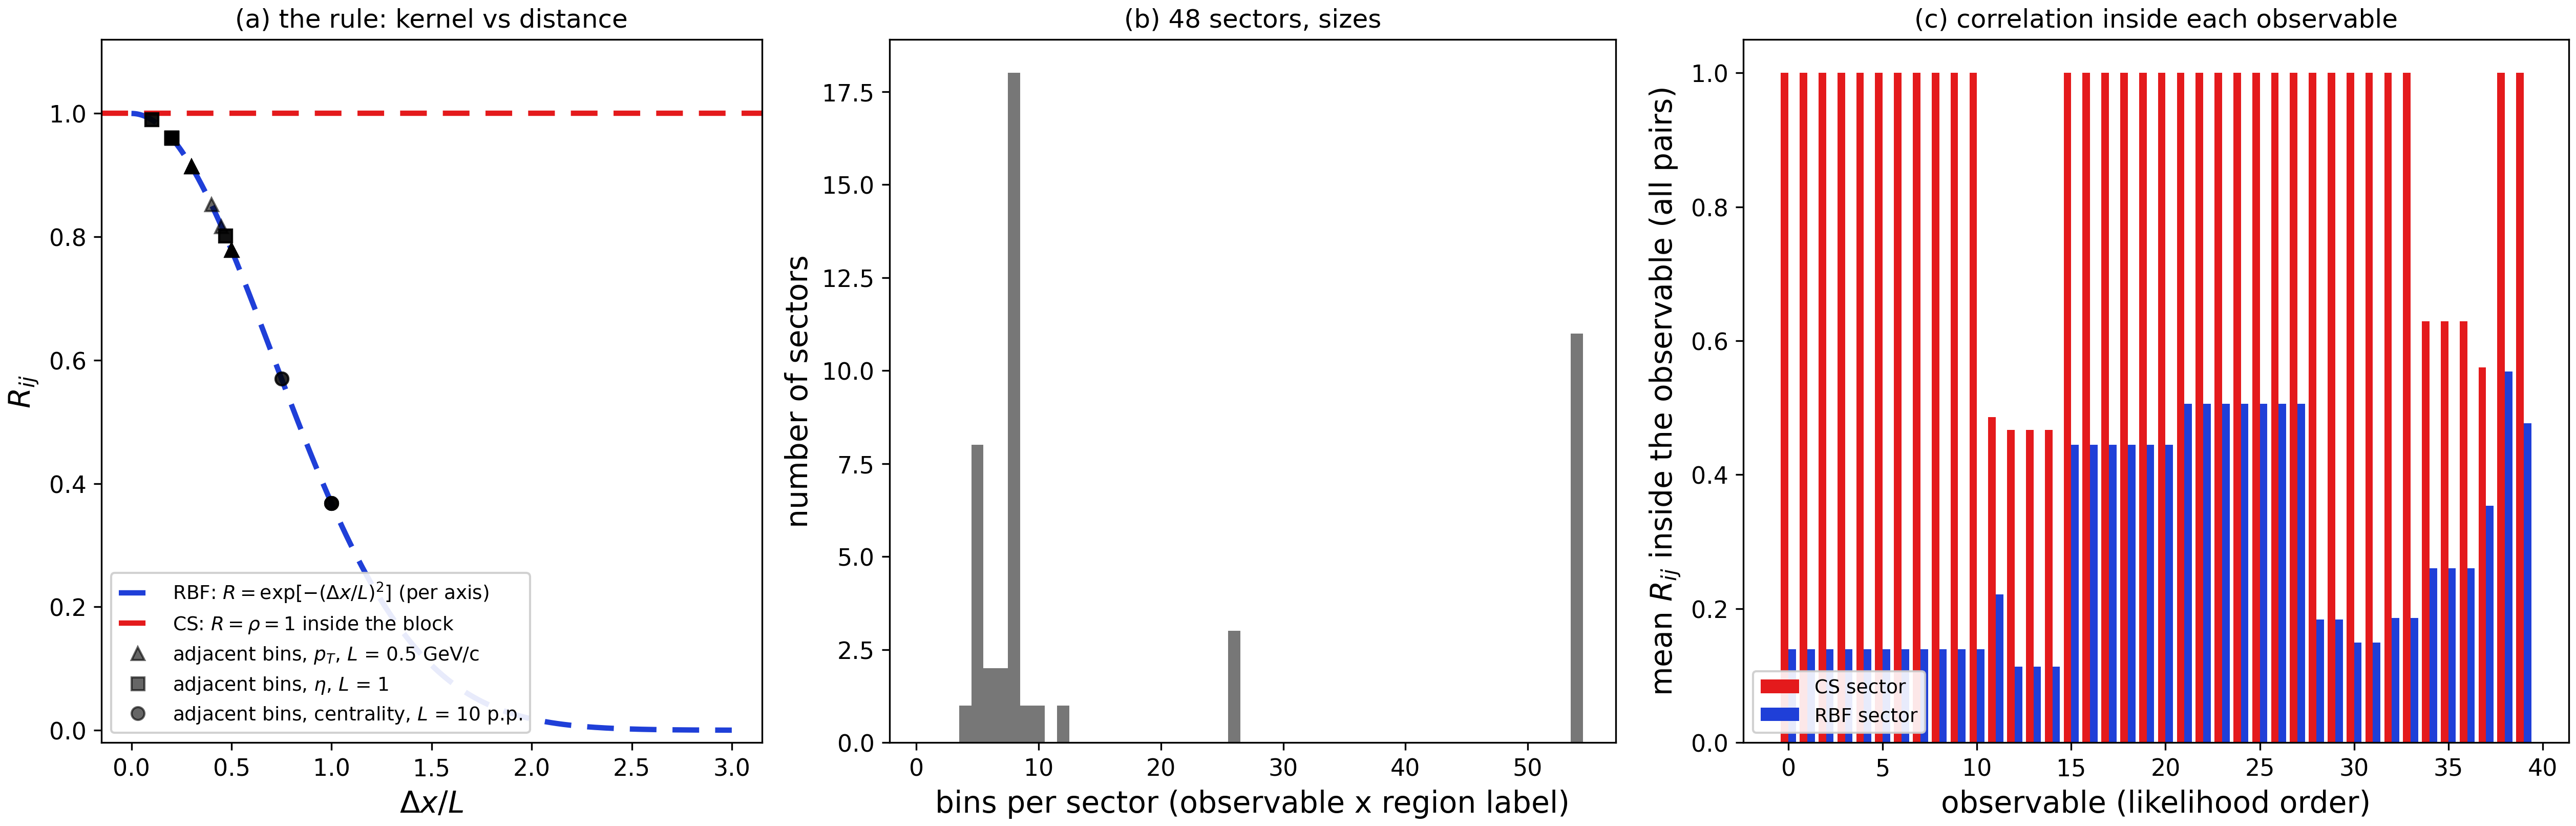
\includegraphics[width=\linewidth]{fig/I1-covariance__sector__cs-rbf.png}
\caption{(a) A regra: $R$ contra $\Delta x/L$, com o espaçamento entre bins adjacentes de cada observável; no CS, $R=1$
dentro do setor. (b) Tamanho dos \valNsectors{} setores (o pico em 54 são as 11 classes do PHOBOS $dN/d\eta$). (c)
$\langle R\rangle$ dentro de cada observável, CS sector e RBF sector.}
\end{figure}
\begin{figure}[H]
\centering
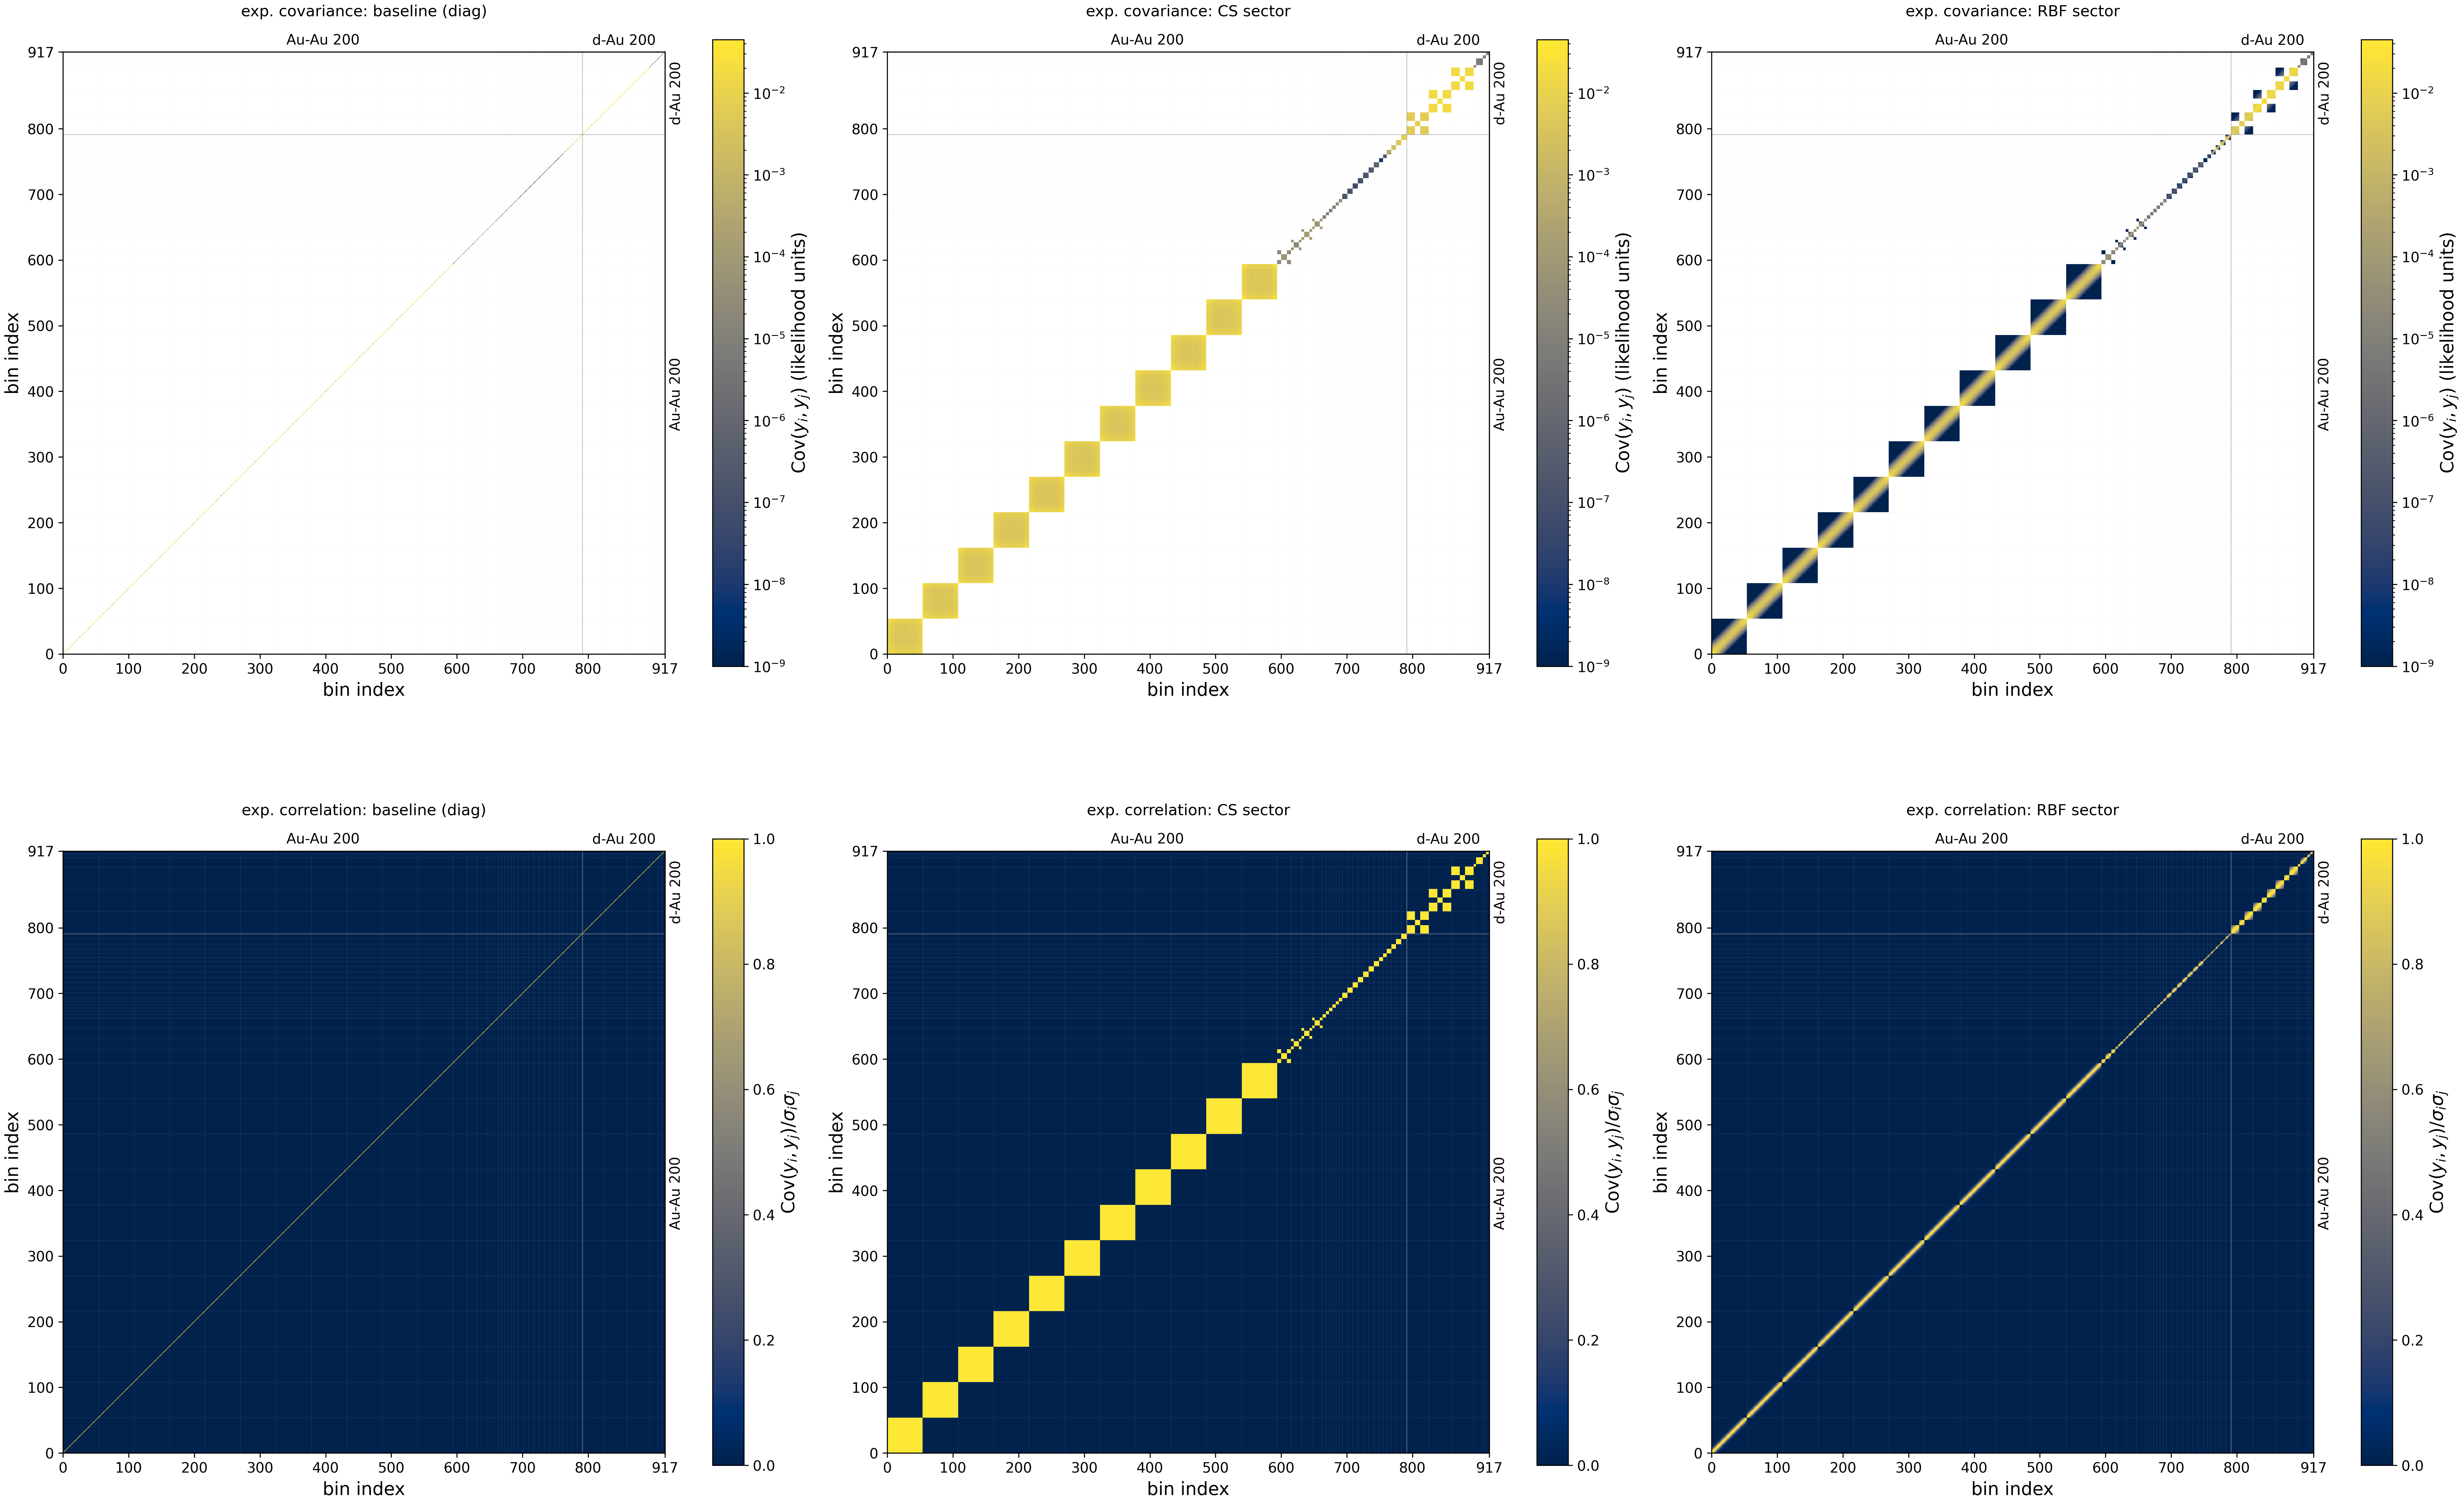
\includegraphics[width=\linewidth]{fig/S2-expcov__sector__baseline-cs-rbf.png}
\caption{Covariância (em cima) e correlação (embaixo) nos 917 bins: baseline, CS sector e RBF sector (\texttt{07\_S2-expcov}).}
\end{figure}
A matriz completa ($\valNbins\times\valNbins$) de cada modelo está em
\arq{I1-covariance__sector__cs-rbf__<cs|rbf>__matrix_cov.csv} e \arq{..._matrix.npz}. Ela é reconstruída com o mesmo
código e os parâmetros gravados nas cadeias e confere com as matrizes de \arq{mcmc/02_08_sector_input_correlations/}
(diferença máxima: CS $\valDiffCs$, RBF $\valDiffRbf$).

\section{O que é suposto}
\begin{center}\small
\begin{tabularx}{\linewidth}{@{}Y l l@{}}
\toprule
ingrediente & origem & valor \\
\midrule
definição de setor (observável + região) & \textbf{escolha} & \valNsectors{} setores \\
fronteiras de rapidez & \textbf{escolha} (região do detector) & Tab.\ da Sec.~3.1 \\
lados ``lateral'' unidos num setor & \textbf{escolha implícita} (mesmo rótulo) & --- \\
correlação dentro do setor (CS) & \textbf{escolha} & $\rho=\valRho$ \\
kernel e comprimentos (RBF) & \textbf{escolha} & $\valLpt$\,GeV/$c$; $\valLeta$; $\valLcent$ p.p. \\
setores diferentes, observáveis diferentes, Au-Au $\leftrightarrow$ d-Au & \textbf{escolha} & 0 \\
variância de cada bin & \textbf{calibração} (JETSCAPE), mantida & $\sigma_i$ \\
\bottomrule
\end{tabularx}
\end{center}

\section{Uso na calibração}
\begin{itemize}[nosep]
\item CS sector: \arq{mcmc/02_04_cs_sector/chain-idf-0-cs-observable-region-rho-1-a77902df73a5.hdf}, \valStepsCs{}
(+20\,000 de burn-in); assinatura \texttt{\valSigCs}.
\item RBF sector: \arq{mcmc/02_05_rbf_sector/chain-idf-0-rbf-observable-a873ae558cc9.hdf}, \valStepsRbf{} (+20\,000);
assinatura \texttt{\valSigRbf}.
\item As figuras usam os primeiros 20\,000 passos de produção (pastas 01--07 desta proposta).
\end{itemize}

\section{Limitações}
\begin{itemize}[nosep]
\item \textbf{Sem correlação entre observáveis}: um erro de normalização comum a várias classes de centralidade (o que
a proposta 3 mede para o PHOBOS) fica fora do modelo. No CS sector, as 11 classes do PHOBOS $dN/d\eta$ são 11 setores
independentes.
\item \textbf{Laterais unidas}: o lado de trás e o da frente de um observável dividido formam um setor só. No CS isso dá
$\rho=1$ entre $\eta<-2$ e $\eta>2$. No RBF, a distância já torna essa correlação desprezível.
\item \textbf{Assinatura}: as cadeias gravam \texttt{covariance\_signature\_matches = False}. A matriz recalculada a partir
dos arquivos de dados não é idêntica bit a bit à usada na cadeia (os $\sigma$ vêm de \texttt{bayes\_exp}, e as versões do
numpy diferem). A reconstrução aqui usa os $\sigma_i$ de \texttt{bin\_index.csv}.
\end{itemize}

\appendix
\section{Incertezas da calibração bin a bin}\label{ap:sigma}
$\sigma_i$ no espaço da verossimilhança. $dN/d\eta$: em \% (log). Demais: em unidades de $10^{-3}$ (absolutas). Formato:
centro do bin: $\sigma_i$. Com a regra da Sec.~3, estes valores determinam a matriz inteira.
\par\medskip
{\scriptsize\tabin{tab/sigma.tex}}

\end{document}
